\documentclass[nochap]{apuntes}

\title{Hoja 1 Autámatas y Lenguajes}
\author{Víctor de Juan Sanz}
\date{2014}


\begin{document}
\maketitle
\section{Autómatas finitos y lenguajes regulares}
\begin{problem}[1]
Dise\~na expresiones regulares para los siguientes lenguajes:
\ppart $L = \{a^nb^m : n + m \text{es impar}\}.$
\ppart Conjunto de n\'umeros binarios que contienen la subcadena $"1010"$

\ppart Identificadores de un lenguaje de programaci\'on que empiezan con el s\'imbolo @, seguido de una letra min\'uscula y cualquier combinaci\'on de letras min\'usculas o n\'umeros.

\solution

\spart $\left[ (aa)*.a.(bb)* \right] + \left[ (aa)*.(bb)*.b\right]$

\spart
$(0+1)*.(1010).(0+1)*$

\spart
Definimos $\mathcal{M} = a+b+c+d+e+f+...$ todas las letras min\'usculas y \\
$\mathcal{N} = 1+2+3+4+5+6+7+8+9+0$

Entonces, la expresión regular que genera el lenguaje es: 

$@.(\mathcal{m}).(\mathcal{M}+\mathcal{N})*$



\end{problem}

\begin{problem}[2]
Diseña un autómata finito (determinista o no determinista) que reconozca cada uno de
los siguientes lenguajes:
\ppart Conjunto de números binarios que contienen la subcadena 1010.
\ppart Identificadores de un lenguaje de programación que empiezan con el símbolo @, seguido de una letra minúscula y cualquier combinación de letras minúsculas o números.

\solution

\spart
Donde el $*$ significa cualquier símbolo del alfabeto.\\


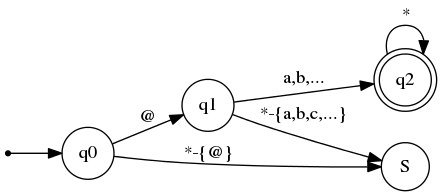
\includegraphics[scale=0.75]{data/png/1_2_a.png}


\spart

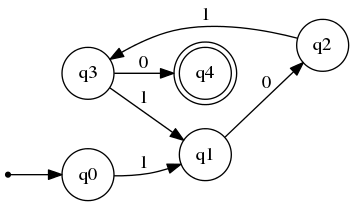
\includegraphics[scale=0.75]{data/png/1_2_b.png}

\end{problem}

\begin{problem}[3]
 Indica cuál es el lenguaje aceptado por el siguiente autómata:
\solution

Vamos a expresar el lenguaje como unión de tres lenguajes aceptados por el autómata:

\begin{itemize}
\item $L_1 = \{b^na \tq n≥1\}$
\item $L_2 = \{b^nab^m \tq m,n≥1\}$
\item $L_3 = \{b^lab^mab^n \tq l,m,n≥1\}$
\end{itemize}

Entonces tenemos $\mathcal{L} = \{b^nab^m \tq n≥1,m≥0\} ∪ \{b^nab^mab^l \tq l,n≥1,m≥0\}$
\end{problem}


\begin{problem}[4]
Construye un autómata finito determinista que acepte cadenas sobre el alfabeto {0, 1} que representen números enteros múltiplos de 5 expresados en representación binaria.
\solution

%\includegraphics[scale=0.75]{data/png/1_4.png}
\end{problem}

\begin{problem}[5]
Para el autómata, encuentra δ*(q0, 1011) y δ*(q1, 01).
\solution

$$δ*(q_0, 1011) = q_2$$

$$δ*(q1, 01) = q_1$$

\end{problem}

\begin{problem}[6]
Construye una autómata finito no determinista con tres estados que acepte el lenguaje $L = {ab, abc}*.$

¿Es posible en menos de 3 estados?
\solution
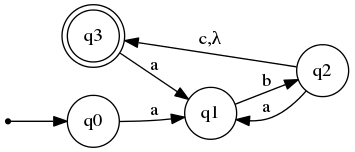
\includegraphics[scale=0.75]{data/png/1_6.png}

Con un autómata que no utilice pila es imposible definirlo con únicamente 2 estados.
\end{problem}

\section{Autómatas a pila y gramáticas independientes del contexto.}
\begin{problem}[1]
Diseña una gramática independiente del contexto que genere el lenguaje de los números capicúa formados con el alfabeto $∑ = \{0, 1, 2, 3, 4, 5, 6, 7, 8, 9\}.$ Los números de una sola cifra no se consideran capicúa.

\solution

\begin{tabular}{cc}
S -> & 0 S 0 \\
S -> & 1 S 1 \\
S -> & 2 S 2 \\
S -> & 3 S 3 \\
S -> & 4 S 4 \\
S -> & 5 S 5 \\
S -> & 6 S 6 \\
S -> & 7 S 7 \\
S -> & 8 S 8 \\
S -> & 9 S 9 \\
\end{tabular}

\end{problem}


\begin{problem}[2]
Diseña una gramática independiente del contexto que genere el lenguaje de los números formados con el alfabeto $\sum = \{0, 1, 2, 3, 4, 5, 6, 7, 8, 9\} $ que tengan el mismo número de dígitos pares e impares. Puede suponerse por simplicidad que los números pueden tener ceros a la izquierda.

\solution

\begin{tabular}{cl}
S ->& PSI\\
S ->& ISP\\
P ->& 0 | 2 | 4 | 6 | 8\\
I ->& 1 | 3 | 5 | 7 | 9
\end{tabular}

\end{problem}

\begin{problem}[3]
Diseña un autómata a pila que reconozca el lenguaje del ejercicio 1.
\solution

Introducimos la notación $A_b^c = \{b,A,c\}$

Por facilitar el dibujo, defino los siguientes símbolos (siendo $z$ el símbolo vacío): 
\begin{itemize}
\item $A=\{0,1,2,3,4,5,6,7,8,9\}$
\item $B=\{z,0,1,2,3,4,5,6,7,8,9\}$
\end{itemize}

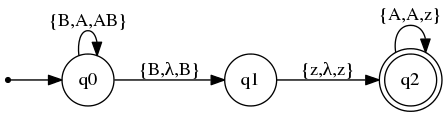
\includegraphics[scale=0.75]{data/png/2_3.png}

\end{problem}

\begin{problem}[4]
Demustra que la gramática es ambigüa
\begin{tabular}{cl}
S &$\to$ AB | aaB\\
A &$\to$ a | Aa\\
B &$\to$ b
\end{tabular}

\solution

Aunque pueda haber ejemplos más complejos, 

\begin{tabular}{c}	
$S\to AB\to aB \to ab$\\
$S\to AB\to Ab \to ab$
\end{tabular}

\end{problem}

\begin{problem}[5]
 Encuentra una gramática independiente del contexto para el siguiente lenguaje:

$$L = \{a^nww^Rb^n : w ∈ {a, b}*, n ≥ 1\}$$

\solution

\begin{tabular}{cl}	
S $\to$& aXb\\
X $\to$& aXa | bXb | λ
\end{tabular}
\end{problem}

\begin{problem}[6]
Indica cuál es el lenguaje aceptado por el siguiente autómata a pila:

A = ({q₀, q₁,q₂}, {a, b}, {a, b, z}, δ, q₀, z, {q₂})\\
δ(q₀, a, z) = {(q₁, a), (q₂, λ)}\\
δ(q₁, b, a) = {(q₁, b)}\\
δ(q₁, b, b) = {(q₁, b)}\\
δ(q₁, a, b) = {(q₂, λ)}


\solution

El dibujo del autómata (que hace más fácil la resolución) es el siguiente (utilizando la notación anterior):

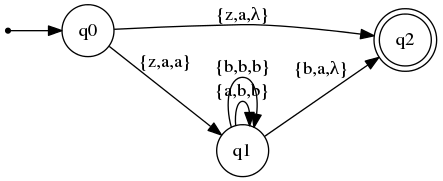
\includegraphics[scale=0.75]{data/png/2_6.png}


El lenguaje aceptado por este autómata es: $$L = \{ab^na\tq n≥1\} ∪ \{a\}$$

\end{problem}


\end{document}
